%2023-April Session-04-10-2023-shift-2-1-15
\let\negmedspace\undefined
\let\negthickspace\undefined
\documentclass[journal]{IEEEtran}
\usepackage[a5paper, margin=10mm, onecolumn]{geometry}
%\usepackage{lmodern} % Ensure lmodern is loaded for pdflatex
\usepackage{tfrupee} % Include tfrupee package

\setlength{\headheight}{1cm} % Set the height of the header box
\setlength{\headsep}{0mm}     % Set the distance between the header box and the top of the text

\usepackage{gvv-book}
\usepackage{gvv}
\usepackage{cite}
\usepackage{amsmath,amssymb,amsfonts,amsthm}
\usepackage{algorithmic}
\usepackage{graphicx}
\usepackage{textcomp}
\usepackage{xcolor}
\usepackage{txfonts}
\usepackage{listings}
\usepackage{enumitem}
\usepackage{mathtools}
\usepackage{gensymb}
\usepackage{comment}
\usepackage[breaklinks=true]{hyperref}
\usepackage{tkz-euclide} 
\usepackage{listings}
% \usepackage{gvv}                                        
\def\inputGnumericTable{}                                 
\usepackage[latin1]{inputenc}                                
\usepackage{color}                                            
\usepackage{array}                                            
\usepackage{longtable}                                       
\usepackage{calc}                                             
\usepackage{multirow}                                         
\usepackage{hhline}                                           
\usepackage{ifthen}                                           
\usepackage{lscape}

\renewcommand{\thefigure}{\theenumi}
\renewcommand{\thetable}{\theenumi}
\setlength{\intextsep}{10pt} % Space between text and floats


\numberwithin{equation}{enumi}
\numberwithin{figure}{enumi}
\renewcommand{\thetable}{\theenumi}

% Marks the beginning of the document
\begin{document}
\bibliographystyle{IEEEtran}

\title{Assignment-3}
\author{EE24BTECH11049}

% \maketitle
% \newpage
% \bigskip
{\let\newpage\relax\maketitle}

\section*{MCQ}
\begin{enumerate}

    %1st Question
    \item 
    If the coefficients of $x$ and $x^2$ in $(1 + x)^p$ $(1 - x)^q$ are $4$ and $-5$ respectively, then $2p + 3q$ is equal to

    \hfill{\brak{\text{2023-Apr}}}

    \begin{enumerate}
    \begin{multicols}{4}
        \item $60$
        \item $63$
        \item $66$
        \item $69$
    \end{multicols}
    \end{enumerate}

    %2nd Question 
    \item 
    let $A = \cbrak{2, 3, 4}$ and $B =  \cbrak{8, 9, 12}$. . Then the number of elements in the relation $R = \cbrak{\brak{\brak{a_1, b_1}, \brak{a_2, b_2}} \in \brak{A \times B, A \times B} : a_1 \text{ divides } b_2 \text{ and } a_2 \text{ divides } b_1}$ is 

    \hfill{\brak{\text{2023-Apr}}}

    \begin{enumerate}
    \begin{multicols}{4}
        \item $18$
        \item $24$
        \item $12$
        \item $36$
    \end{multicols}
    \end{enumerate}

    %3rd Question 
    \item 
    Let time image of the point $\vec{P}\brak{1, 2, 6}$ n the plane passing through the points $\vec{A}\brak{1, 2, 0}$, $\vec{B}\brak{1, 4, 1}$ and $\vec{C}\brak{0, 5, 1}$ be $\vec{Q}\brak{\alpha, \beta, \gamma}$. Then $\brak{\alpha^2 + \beta^2 + \gamma^2}$ is equal to

    \hfill{\brak{\text{2023-Apr}}}

    \begin{enumerate}
    \begin{multicols}{4}
        \item $70$
        \item $76$
        \item $62$
        \item $65$
    \end{multicols}
    \end{enumerate}

    %4th Question 
    \item 
    The statement $\sim\sbrak{p \lor \brak{\sim \brak{p \land q}}}$ is equivalent to

    \hfill{\brak{\text{2023-Apr}}}

    \begin{enumerate}
    \begin{multicols}{4}
        \item $\brak{\sim\brak{p \land q}} \land q$
        \item $\sim\brak{p \lor q}$
        \item $\sim\brak{p \land q}$
        \item $\brak{p \land q} \land \brak{\sim }$
    \end{multicols}   
    \end{enumerate}

    %5th Question 
    \item 
    let 
    \begin{align*}
        S = \cbrak{x \in \brak{-\frac{\pi}{2}, \frac{\pi}{2}} : 9^{1-\tan^2 x} + 9^{\tan^2 x} = 10} \text{ and } b = \sum_{x \in S} \tan^2 {\brak{\frac{x}{3}}},
   \end{align*}
   then $\frac{1}{6}\brak{\beta -14}^2$ is equal to

    \hfill{\brak{\text{2023-Apr}}}

    \begin{enumerate}
    \begin{multicols}{4}
        \item $16$
        \item $32$
        \item $8$
        \item $64$
    \end{multicols}
    \end{enumerate}

    %6th Question 
    \item
    If the points $\vec{P}$ and $\vec{Q}$ are respectively the circumcenter and the orthocentre of a $\Delta ABC$, the $\overline{\vec{PA}} + \overline{\vec{PB}} + \overline{\vec{PC}}$ is equal to

    \hfill{\brak{\text{2023-Apr}}}

    \begin{enumerate}
    \begin{multicols}{4}
        \item $2\overline{\vec{QP}}$
        \item $\overline{\vec{QP}}$
        \item $2\overline{\vec{PQ}}$
        \item $\overline{\vec{PQ}}$
    \end{multicols}
    \end{enumerate}

    \begin{figure}[H]
        \centering
        \begin{tikzpicture}
            \draw[thick] (0, 0) -- (2, 0);
            \draw[thick] (0, 0) -- (1, 1.732);
            \draw[thick] (1, 1.732) -- (2, 0);

            \node[below] at (0, 0){$\vec{B}$};
            \node[below] at (2, 0){$\vec{C}$};
            \node[above] at (1, 1.732){$\vec{A}$};
            \node[left] at (0.9, 0.8){$\vec{P}$};
            \node[right] at (1.1, 0.6){$\vec{Q}$};
            
            \fill[black] (0.9, 0.8) circle(1pt);
            \fill[black] (1.1, 0.6) circle(1pt);
        \end{tikzpicture}
    \end{figure}

    %7th Question 
    \item 
    Let $\vec{A}$ be the point $\brak{1, 2}$ and $\vec{B}$ be any point on the curve $x^2 + y^2 = 16$. $\vec{f}$ the centre of the locus of the point $\vec{P}$, which divides the line segment $\vec{AB}$ in the ratio $3 : 2$ is the point $\vec{C}\brak{\alpha, \beta}$ then the length of the line segment $\vec{AC}$ is

    \hfill{\brak{\text{2023-Apr}}}

    \begin{enumerate}
    \begin{multicols}{4}
        \item $\frac{6\sqrt{5}}{5}$
        \item $\frac{2\sqrt{5}}{5}$
        \item $\frac{3\sqrt{5}}{5}$
        \item $\frac{4\sqrt{5}}{5}$
    \end{multicols}
    \end{enumerate}

    \begin{figure}[H]
        \centering
        \begin{tikzpicture}
            \draw[thick] (0, 0) circle(2cm);

            \fill[black] (0, 0) circle(1.5pt);
            \fill[black] (0, 2) circle(1.5pt);
            \fill[black] (0.5, 1) circle(1.5pt);

            \node[above] at (0, 2){$\vec{B}\brak{4\cos{\theta}, 4\sin{\theta}}$};
            \node[below] at (0, 0){$\vec{f}\brak{0,0}$};
            \node[above] at (0.5, 1){$\vec{A}\brak{1,2}$};
        \end{tikzpicture}
    \end{figure}

    %8th Question 
    \item  
    Let $m$ be the mean and $\sigma$ be the standard deviation of the distribution
    \begin{table}[H]
        \centering
        \begin{tabular}{|c |c |c |c |c |c |c |}
        
        \hline
             $x_i$ & $0$ & $1$ & $2$ & $3$ & $4$ & $5$ \\
        \hline
             $f_i$ & $k + 2$ & $2k$ & $k^2 - 1$ & $k^2 -1$ & $k^2 +1$ & $k - 3$ \\
        \hline
        \end{tabular}
    \end{table}
    where $\sum f_i = 62$. If $\sbrak{x}$ denotes the greatest integer $\leq x $, then $\sbrak{\mu^2 + \sigma^2}$ is equal to

    \hfill{\brak{\text{2023-Apr}}}

    \begin{enumerate}
    \begin{multicols}{4}
        \item $8$
        \item $7$
        \item $6$
        \item $9$
    \end{multicols}
    \end{enumerate}

    %9th Question
    \item 
    If $S_n = 4 + 11 + 21 + 34 + 50 + \dots$ to $n$ terms, then $\frac{1}{60}\brak{S_{29} - S_9}$ 
    
    \hfill{\brak{\text{2023-Apr}}}

    \begin{enumerate}
    \begin{multicols}{4}
        \item $220$
        \item $227$
        \item $226$
        \item $223$
    \end{multicols}
    \end{enumerate}

    %10th Question 
    \item 
    Eight persons are to be transported from city $A$ to city $B$ in three cars different makes. If each car can accommodate at most three persons, then the number of ways, in which they can be transported, is

    \hfill{\brak{\text{2023-Apr}}}

    \begin{enumerate}
    \begin{multicols}{4}
        \item $1120$
        \item $560$
        \item $3360$
        \item $1680$
    \end{multicols}
    \end{enumerate}

    %11th Question 
    \item 
    If 
    \begin{align*}
        A = \frac{1}{5!6!7!}\myvec{5! & 6! & 7!\\6! & 7! & 8!\\7! & 8! & 9!},
    \end{align*}
    then $\abs{\text{adj}\brak{\text{adj}\brak{2A}}}$ is equal to

    \hfill{\brak{\text{2023-Apr}}}

    \begin{enumerate}
    \begin{multicols}{4}
        \item $2^{16}$
        \item $2^8$
        \item $2^{12}$
        \item $2^{20}$
    \end{multicols}
    \end{enumerate}

    %12th Question 
    \item 
    Let the number $\brak{22}^{2022} + \brak{2022}^{22}$ leave the remainder $\alpha$ when divided by $3$ and $\beta$ when divided by $7$. Then $\brak{\alpha^2 + \beta^2}$ is equal to

    \hfill{\brak{\text{2023-Apr}}}

    \begin{enumerate}
    \begin{multicols}{4}
        \item $13$
        \item $20$
        \item $10$
        \item $5$
    \end{multicols}
    \end{enumerate}

    %13th Question 
    \item 
    let 
    \begin{align*}
        g\brak{x} = f\brak{x} + f\brak{1 - x} \text{ and } f^n\brak{x} > 0, x \in \brak{0, 1}.
    \end{align*}
    If $g$ is decreasing in the interval $\brak{0, \alpha}$ and increasing in the interval $\brak{\alpha, 1}$, then 
    \begin{align*}
        \tan^{-1} {\brak{2\alpha}} + \tan^{-1} {\brak{\frac{\alpha + 1}{\alpha}}}
    \end{align*}
    is equal to

    \hfill{\brak{\text{2023-Apr}}}

    \begin{enumerate}
    \begin{multicols}{4}
        \item $\frac{5\pi}{4}$
        \item $\pi$
        \item $\frac{3\pi}{4}$
        \item $\frac{3\pi}{2}$
    \end{multicols}
    \end{enumerate}

    %14th Question 
    \item 
    For $\alpha, \beta, \gamma, \delta \in \mathbf{N}$, if
    \begin{align*}
         \int \brak{\brak{\frac{x}{e}}^{2x} + \brak{\frac{e}{x}}^{2x}} \log_ex \, dx = \frac{1}{\alpha}\brak{\frac{x}{e}}^{\beta x} - \frac{1}{\gamma}\brak{\frac{e}{x}}^{\delta x} + C, \text{ where } e = \sum_{n = 0}^\infty \frac{1}{n!}
    \end{align*}
    and $C$ is constant of integration, then $\alpha + 2\beta + 3\gamma - 4\delta$ is equal to

    \hfill{\brak{\text{2023-Apr}}}

    \begin{enumerate}
    \begin{multicols}{4}
        \item $4$
        \item $-4$
        \item $-8$
        \item $1$
    \end{multicols}
    \end{enumerate}

    %15th Question 
    \item 
    Let $f$ be a continuous function satisfying
    \begin{align*}
        \int_0^{t^2} \brak{f\brak{x} + x^2} \, dx = \frac{4}{3}t^3, \forall t > 0. 
    \end{align*}
    Then $f\brak{\frac{\pi^2}{4}}$ is equal to

    \hfill{\brak{\text{2023-Apr}}}

    \begin{enumerate}
    \begin{multicols}{4}
        \item $-\pi^2 \brak{1 + \frac{\pi^2}{16}}$
        \item $\pi \brak{1 - \frac{\pi^3}{16}}$
        \item $-\pi \brak{1 + \frac{\pi^3}{16}}$
        \item $\pi^2 \brak{1 - \frac{\pi^3}{16}}$
    \end{multicols}
    \end{enumerate}
    
    
\end{enumerate}
\end{document} 
